\documentclass[draft,caption=numbered]{beamer}
\usetheme[color=screen]{UniBern}

\usepackage{lmodern}
\usepackage[english]{babel}
\usepackage{microtype}
\usepackage{textcomp}
\usepackage[backend=biber, style=alphabetic, url=false]{biblatex}
\addbibresource{../../Documents/library.bib}
\usepackage{graphicx}
\usepackage{caption}
    \captionsetup[figure]{labelformat=empty} % No 'figure' in figures
\usepackage{tikz}
\usepackage[detect-all=true]{siunitx}
\usepackage{csquotes}
\usepackage{animate}
\usepackage{booktabs}
\usepackage[absolute,overlay]{textpos} %for the \source{} command
\usepackage{gitinfo2}
\usepackage{hyperref}

\hypersetup{pdfstartview={Fit}}
\setbeamertemplate{caption}{\insertcaption}
\setbeamertemplate{caption}[numbered]

\newcommand{\imsize}{\linewidth}
\newlength\imagewidth % needed for scalebars
\newlength\imagescale % ditto
\newcommand{\uct}{\si{micro}CT}
\newcommand{\uaf}{\si{micro}AngioFil}

\newcommand{\source}[1]{%http://tex.stackexchange.com/a/48485/828
    \begin{textblock*}{4cm}(8.7cm,8.6cm)%
    \begin{beamercolorbox}[ht=0.5cm,right]{framesource}%
    \tiny\usebeamerfont{framesource}\usebeamercolor[fg]{framesource} Source: {#1}%
    \end{beamercolorbox}%
    \end{textblock*}%
}

% Biblatex: http://tex.stackexchange.com/a/13076/828
% % Format bibliography for beamer
% % http://tex.stackexchange.com/a/10686/828
% \renewbibmacro{in:}{}
% % http://tex.stackexchange.com/a/13076/828
% \AtEveryBibitem{\clearfield{title}}
% \AtEveryBibitem{\clearfield{journaltitle}}
% \AtEveryBibitem{\clearfield{year}}
% \AtEveryBibitem{\clearfield{pages}}
% \AtEveryBibitem{\clearfield{volume}}
% \AtEveryBibitem{\clearfield{number}}
% %http://tex.stackexchange.com/a/40710/828
% \usepackage{xpatch}
% \xpatchbibmacro{month}{%
%   \printtext[parens]%
% }{%
%   \setunit*{\addperiod\space}%
%   \printtext%
% }{}{} 

\subtitle{Brain and lung imaging as examples}
\author[DH]{David Haberthür}
\institute{Institute of Anatomy\\Universität Bern}
\date{February 9, 2017\\Internal seminar\\Version~\gitAbbrevHash}

\useoutertheme{split}

\begin{document}
\title[\si{\micro}CT imaging at ana.unibe.ch]{\si{\micro}CT-imaging at the Institute of Anatomy} % http://tex.stackexchange.com/a/144445/828

\defbeamertemplate{footline}{unibe}
{%
	\usebeamercolor[fg]{page number in head/foot}%
	\usebeamerfont{page number in head/foot}%
	\hspace*{\fill}%
	\insertauthor%
	\hspace*{\fill}%|\hspace*{\fill}%
	\insertshorttitle%
	\hspace*{\fill}%|\hspace*{\fill}%
	v.~\gitAbbrevHash%
	\hspace*{\fill}%|\hspace*{\fill}%
	\insertpagenumber\,/\,\insertpresentationendpage%
	\hspace*{\fill}%
	\vskip2pt%
}
\setbeamertemplate{footline}[unibe]

{
\setbeamertemplate{footline}{} % http://tex.stackexchange.com/a/18829/828
\begin{frame}
  \titlepage
\end{frame}
}
\addtocounter{framenumber}{1}

\begin{frame}{Contents}
	\tableofcontents
\end{frame}

\section{Overview}
\begin{frame}{Backstory}
    \begin{itemize}
        \item Lung fibrosis grading \cite{Ashcroft1988a}
        \item \emph{Correct} sampling for proper assessment
        \item \uct is a tool to help grade fibrosis
        \begin{itemize}
            \item Detect and grade fibrosis
            \item Get indications where to perform the sampling
        \end{itemize}
        \item Cancer metastasis (\SI{2}{year} after radiation treatment fibrosis is induced)
        \item Cancer treatment
        \begin{itemize}
            \item Antiangiogenesis (failed)
            \item Radiation therapy, namely MRT \cite{Bronnimann2016} (probably better citation needed)!
        \end{itemize}
    \end{itemize}
\end{frame}


\begin{frame}{Stories}
    \begin{itemize}
        \item  Overview of metastatis (Ochsenbein sample)
        \item Fibrosis grading (3View/uCT)
        \item Grenoble brains, assessing different parameters `easily'.
    \end{itemize}
\end{frame}

\section{\uct}
\renewcommand{\imsize}{0.618\linewidth}
\begin{frame}{Theory}
    \centering
    \begin{figure}
    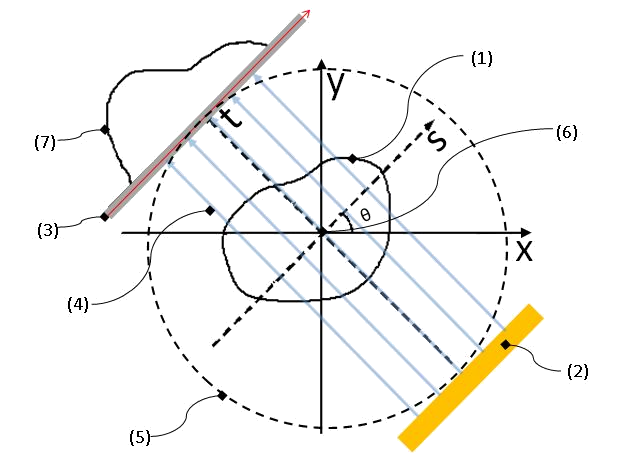
\includegraphics[width=\imsize]{img/CT_PRINCI_PB}
    \caption[CT]{Parallel beam CT.
        1: Object
        2: Parallel beam light source
        3: Screen
        4: Transmitted beam
        5: Datum circle
        6: Origin
        7: 1D image}
    \end{figure}
    \source{\href{https://commons.wikimedia.org/wiki/File:CT_PRINCI_PB.jpg}{enwp.org/tomography}}
\end{frame}

\subsection{examples}
\begin{frame}{Zebrafish}
    \renewcommand{\imsize}{\linewidth}%
    \begin{figure}%
        \centering%
        \pgfmathsetlength{\imagewidth}{\imsize}%
        \pgfmathsetlength{\imagescale}{\imagewidth/1651}%
        \def\x{1020}% scalebar-x starting at golden ratio of image width of 1651px = 1020
        \def\y{391}% scalebar-y at 90% of image height of 434px = 391
        \begin{tikzpicture}[x=\imagescale,y=-\imagescale]%
            \node[anchor=north west, inner sep=0pt, outer sep=0pt] at (0,0) {\includegraphics[width=\imagewidth]{img/{{zebrafish_rec_voi_side}}}};
            % 1615px = 35.48 > 100px = 2198um > 23px = 500um, 5px = 100um
            %\draw[|-|,blue,thick] (20,154) -- (1634,127) node [sloped,midway,above,fill=white,semitransparent,text opacity=1] {\SI{35.487480000000005}{\milli\meter} (1615px) TEMPORARY!};
            \draw[|-|,ultra thick] (\x,\y) -- (\x+234.19,\y) node [midway,above] {\SI{5}{\milli\meter}};
        \end{tikzpicture}%
        \caption{Visualization of a tomographic scan of a zebrafish, fixed in \SI{4}{\percent} PFA.}%
    \end{figure}%
\end{frame}

\begin{frame}{Zebrafish}
    \renewcommand{\imsize}{0.618\linewidth}%
    \begin{figure}%
        \centering%
        \pgfmathsetlength{\imagewidth}{\imsize}%
        \pgfmathsetlength{\imagescale}{\imagewidth/1604}%
        \def\x{991}% scalebar-x starting at golden ratio of image width of 1604px = 991
        \def\y{816}% scalebar-y at 90% of image height of 907px = 816
        \def\mag{4}    % magnification of inset
        \def\size{75}  % size of inset
        \def\shadow{4} % shadow parameter for scalebar
        \begin{tikzpicture}[x=\imagescale,y=-\imagescale, spy using outlines={rectangle, magnification=\mag, size=\size, connect spies}]
            \begin{scope}
                \clip (0,0) rectangle (1604,907);
                %\clip (802.0,453.5) circle (453.5);
                \node[anchor=north west, inner sep=0pt, outer sep=0pt] at (0,0) {\includegraphics[width=\imagewidth]{./img/{{zebrafish_rec_voi_top_right}}}};
            \end{scope}
            %\spy [red] on (1304,607) in node at (0,0) [anchor=north west];
            % 1726px = 35.63mm > 100px = 2064um > 24px = 500um, 5px = 100um
            %\draw[|-|,blue,thick] (32,40) -- (1555,851) node [sloped,midway,above,fill=white,semitransparent,text opacity=1] {\SI{35.63}{\milli\meter} (1726px) TEMPORARY!};
            \draw[|-|,thick] (\x+\shadow,\y+\shadow) -- (\x+24+\shadow,\y+\shadow) node [midway, above] {\SI{500}{\micro\meter}};
            \draw[|-|,white,thick] (\x,\y) -- (\x+24,\y) node [midway,above] {\SI{500}{\micro\meter}};
            %\draw[color=red, anchor=south west] (0,907) node [fill=white, semitransparent] {Legend} node {Legend};
        \end{tikzpicture}%
        \caption{Visualization of a tomographic scan of a whole zebrafish, fixed in \SI{4}{\percent} PFA.}%
    \end{figure}%
\end{frame}

\begin{frame}{Rat head}
    \renewcommand{\imsize}{\linewidth}%
    \begin{figure}%
        \centering%
        \pgfmathsetlength{\imagewidth}{\imsize}%
        \pgfmathsetlength{\imagescale}{\imagewidth/1400}%
        \def\x{865}% scalebar-x starting at golden ratio of image width of 1400px = 865
        \def\y{560}% scalebar-y at 90% of image height of 622px = 560
        \def\mag{4}    % magnification of inset
        \def\size{75}  % size of inset
        \def\shadow{4} % shadow parameter for scalebar
        \begin{tikzpicture}[x=\imagescale,y=-\imagescale, spy using outlines={rectangle, magnification=\mag, size=\size, connect spies}]
            \begin{scope}
                \clip (0,0) rectangle (1400,622);
                %\clip (700.0,311.0) circle (311.0);
                \node[anchor=north west, inner sep=0pt, outer sep=0pt] at (0,0) {\includegraphics[width=\imagewidth]{./img/{{ratwholehead_rec_side}}}};
            \end{scope}
            %\spy [red] on (1100,322) in node at (0,0) [anchor=north west];
            % 1358px = 47.76mm > 100px = 3517um > 14px = 500um, 3px = 100um
            %\draw[|-|,blue,thick] (23,291) -- (1380,311) node [sloped,midway,above,fill=white,semitransparent,text opacity=1] {\SI{47.76}{\milli\meter} (1358px) TEMPORARY!};
            \draw[|-|,thick] (\x+\shadow,\y+\shadow) -- (\x+14+\shadow,\y+\shadow) node [midway, above] {\SI{500}{\micro\meter}};
            \draw[|-|,white,thick] (\x,\y) -- (\x+14,\y) node [midway,above] {\SI{500}{\micro\meter}};
            %\draw[color=red, anchor=south west] (0,622) node [fill=white, semitransparent] {Legend} node {Legend};
        \end{tikzpicture}%
        \caption{Visualization of a tomographic scan of a rat head, instilled with \uaf and fixed in \SI{4}{\percent} PFA.}%
    \end{figure}%
\end{frame}

\begin{frame}{Spider}
\end{frame}

\begin{frame}{Rat brain vessels}
will be important later on with Grenoble brains
\centering
        \pgfmathsetlength{\imagewidth}{\imsize}%
        \pgfmathsetlength{\imagescale}{\imagewidth/1950}%
        \def\x{1205}% scalebar-x starting at golden ratio of image width of 1950px = 1205
        \def\y{1230}% scalebar-y at 90% of image height of 1367px = 1230
        \begin{tikzpicture}[x=\imagescale,y=-\imagescale]
            \node[anchor=north west, inner sep=0pt, outer sep=0pt] at (0,0) {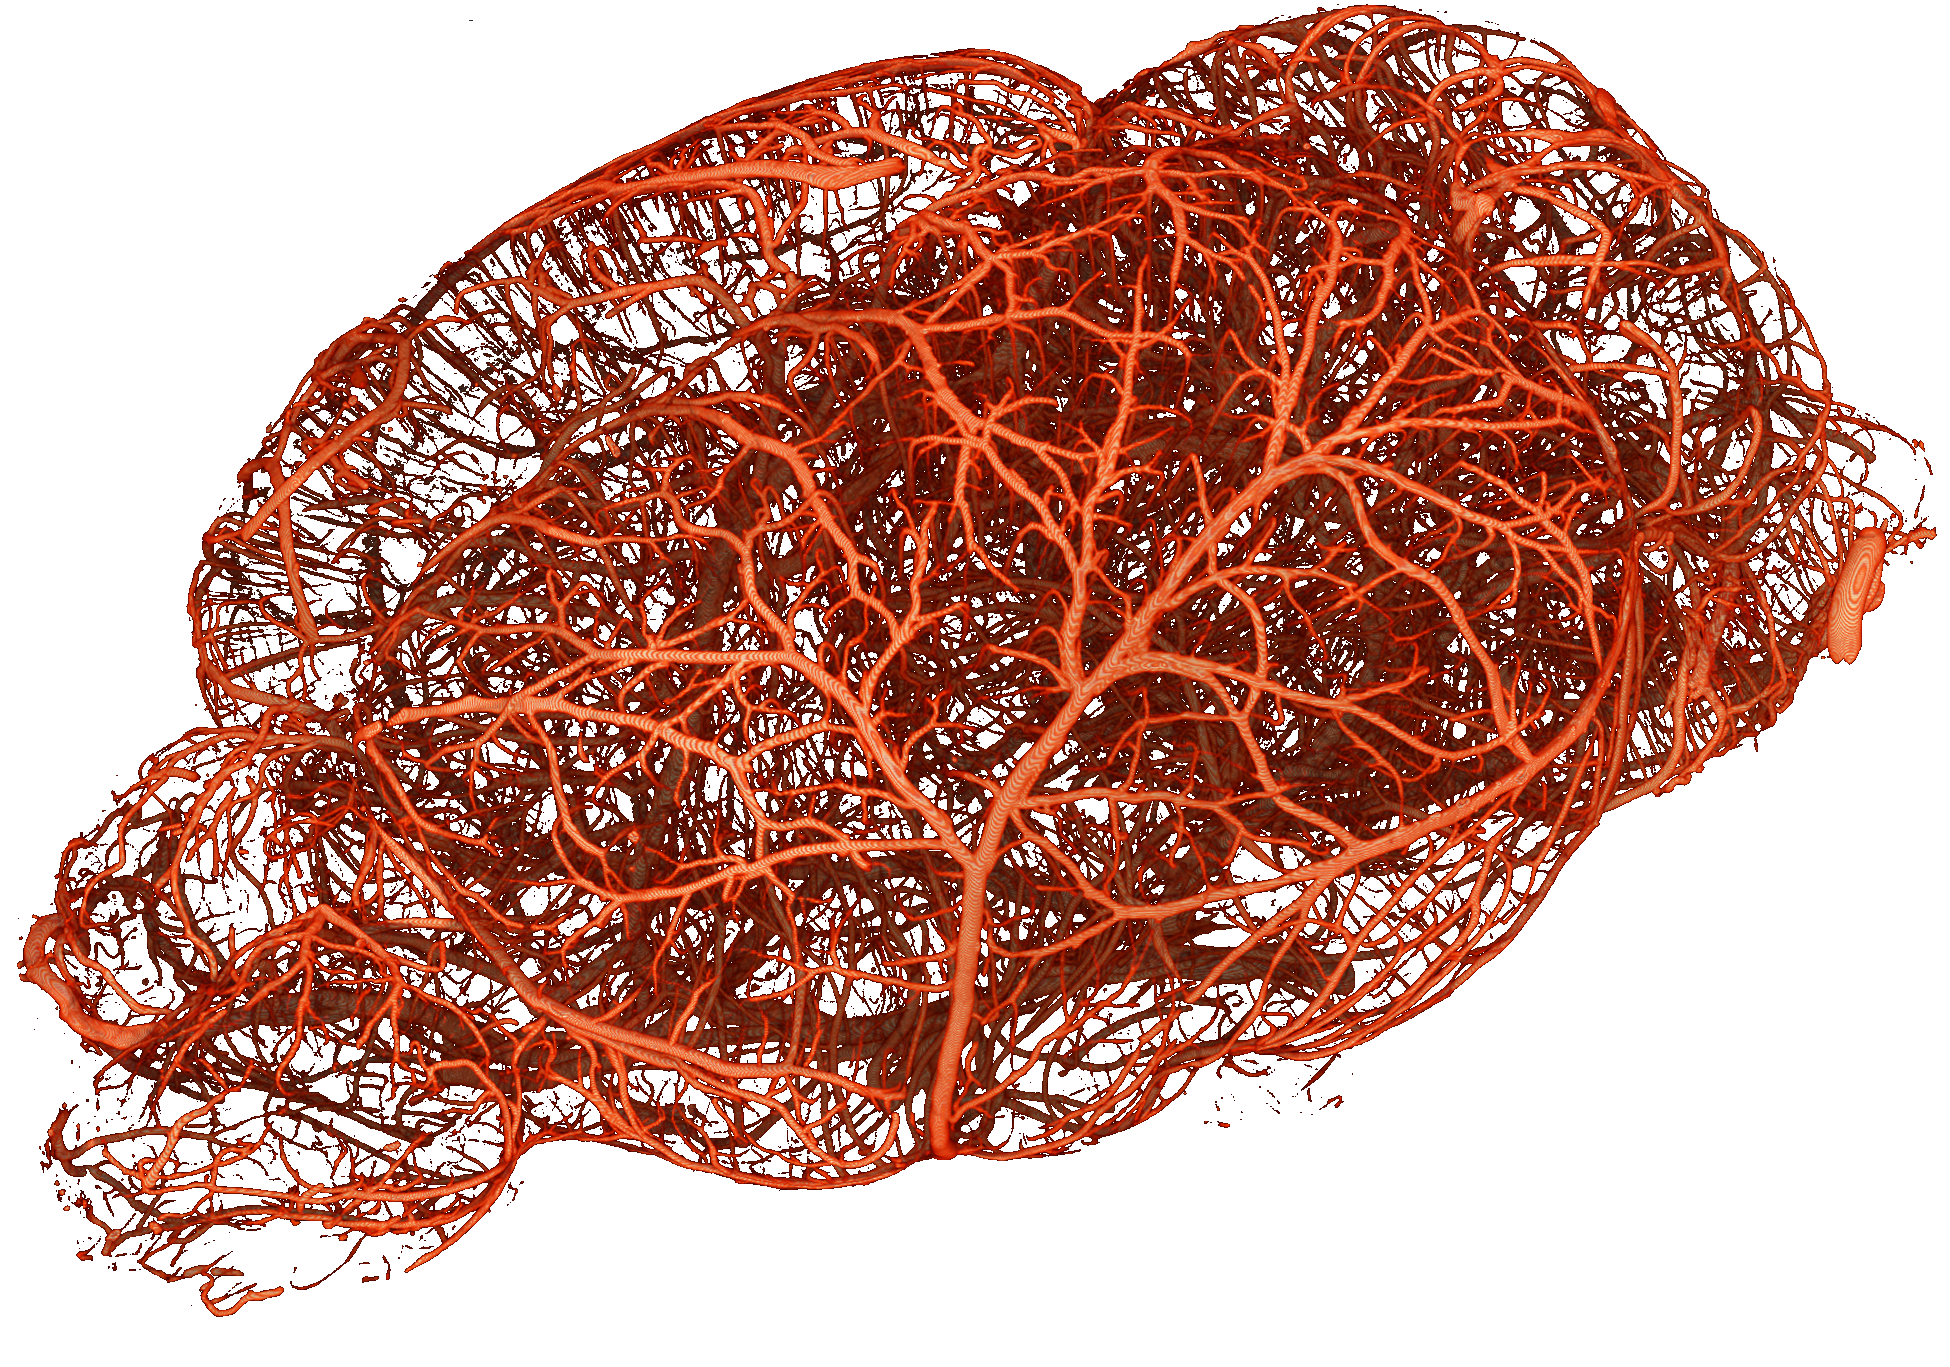
\includegraphics[width=\imagewidth]{img/Ebene_25}};
            % 1949px = 20.0mm > 100px = 1026um > 49px = 500um, 10px = 100um
            %\draw[|-|,blue,thick] (39,1222) -- (1722,239) node [sloped,midway,above,fill=white,semitransparent,text opacity=1] {\SI{20.0}{\milli\meter} (1949px) TEMPORARY!};
            \draw[|-|, thick] (\x,\y) -- (\x+97,\y) node [midway,above] {\SI{1}{\milli\meter}};
            \node [anchor=west] (cb) at (50,150) {Cerebellum};
            \draw [double arrow=5pt colored by white and black] (cb) to [out=0, in=160] (1482,144);
            \node [anchor=center] (bs) at (1705,1000) {Brain stem};
            \draw [double arrow=5pt colored by white and black] (bs.north) to [out=90, in=-45] (1705,725);
            \node [anchor=west, text width=5cm, align=center] (ob) at (50,300) {Olfactory bulbs};
            \draw [double arrow=5pt colored by white and black] (ob.south) to [out=-90, in=135] (210,880);
            \draw [double arrow=5pt colored by white and black] (ob.south) to [out=-90, in=45] (298,1116);
        \end{tikzpicture}
\end{frame}

\section{Assessing metastasis load in lungs}
\renewcommand{\imsize}{0.3\linewidth}  
\begin{frame}{Tumor metastasis, Tumor load in lungs, KP-TNIK mice. Top: KO, bottom: WT}
    \centering
    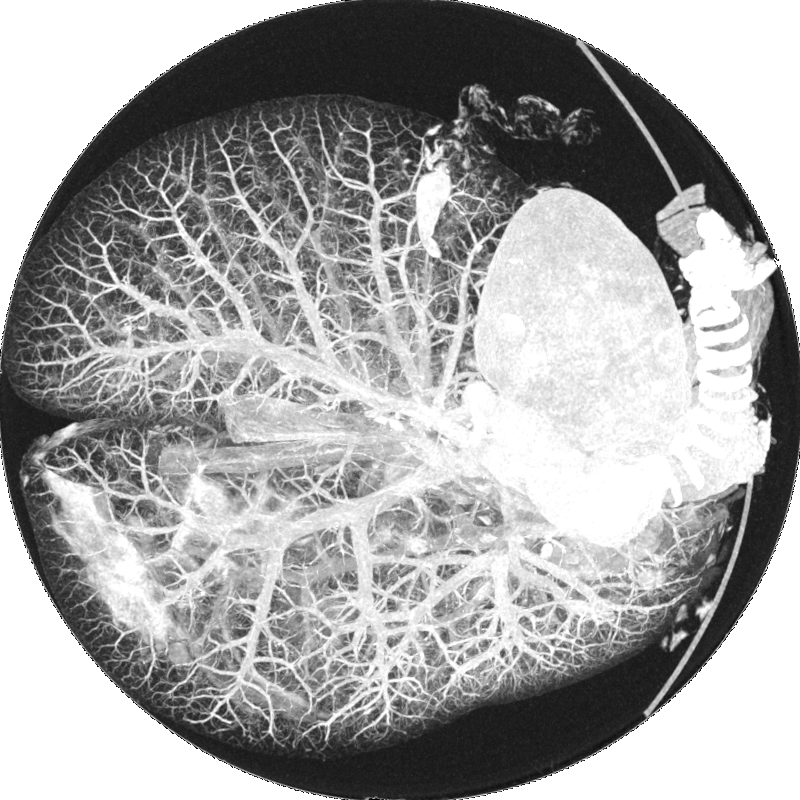
\includegraphics[width=\imsize]{../../Documents/Collaborations/DKF_Lung/Overview/MAX_--11.png}%
    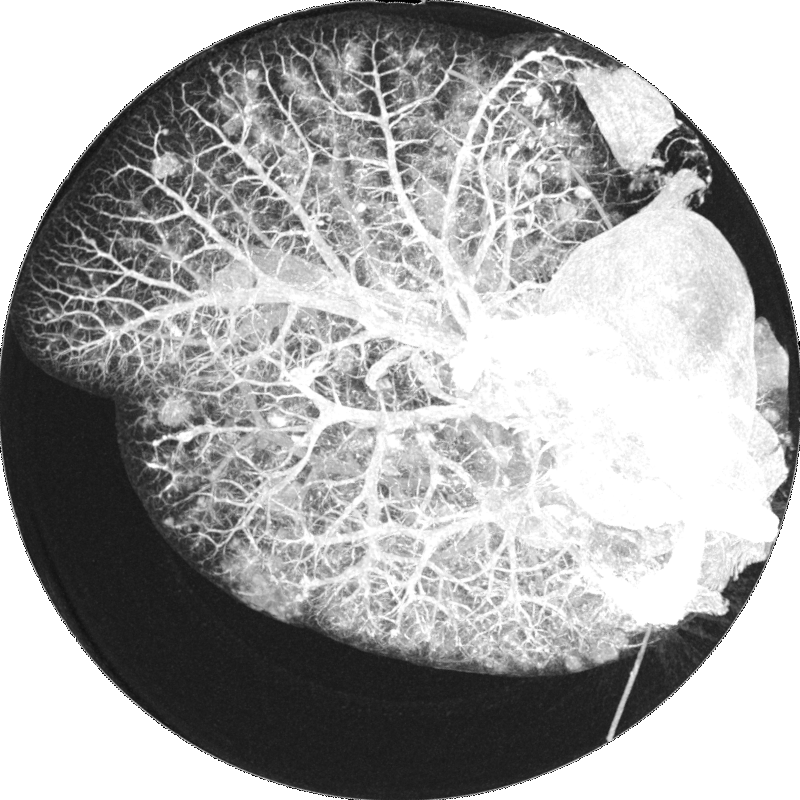
\includegraphics[width=\imsize]{../../Documents/Collaborations/DKF_Lung/Overview/MAX_--12.png}%
    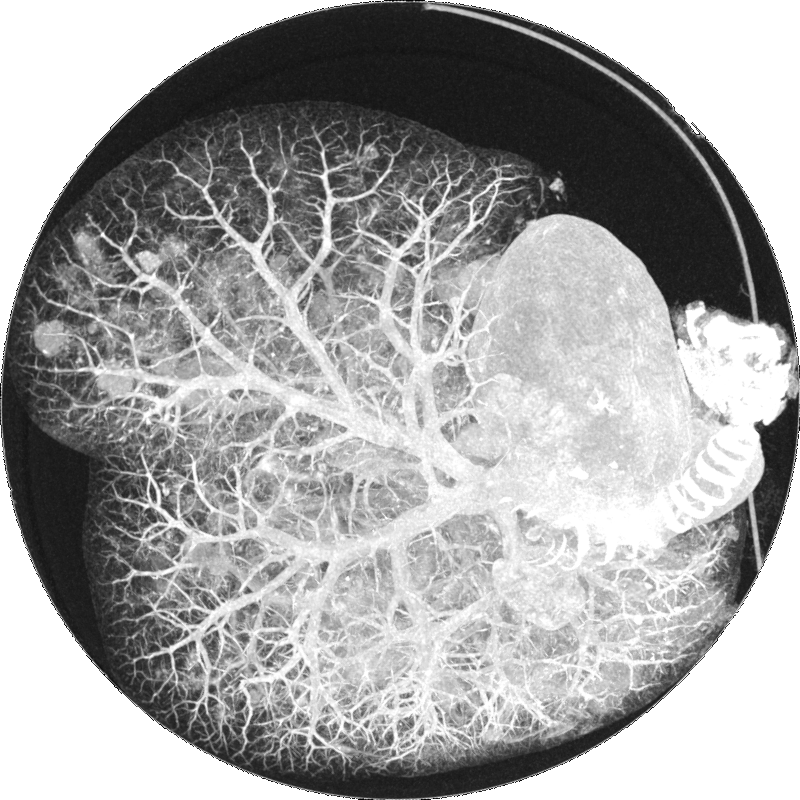
\includegraphics[width=\imsize]{../../Documents/Collaborations/DKF_Lung/Overview/MAX_--13.png}\\%
    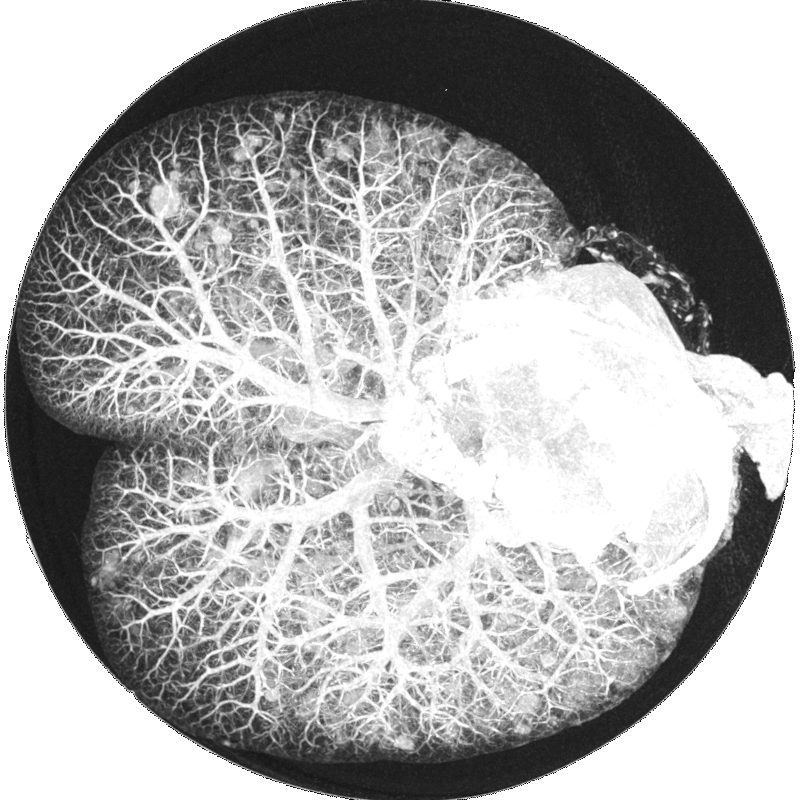
\includegraphics[width=\imsize]{../../Documents/Collaborations/DKF_Lung/Overview/MAX_wt11.png}%
    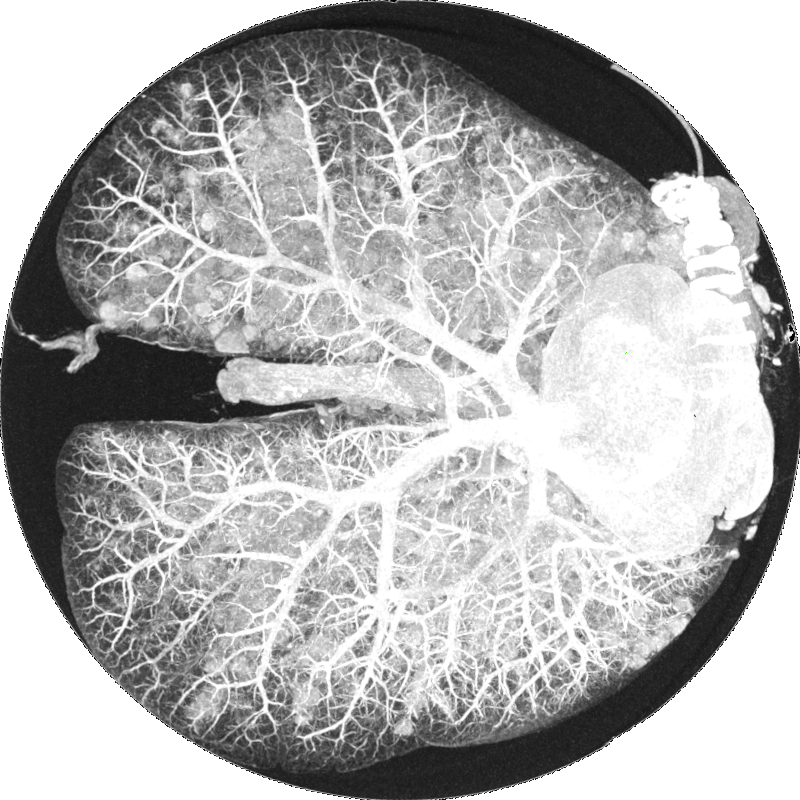
\includegraphics[width=\imsize]{../../Documents/Collaborations/DKF_Lung/Overview/MAX_wt12.png}%
    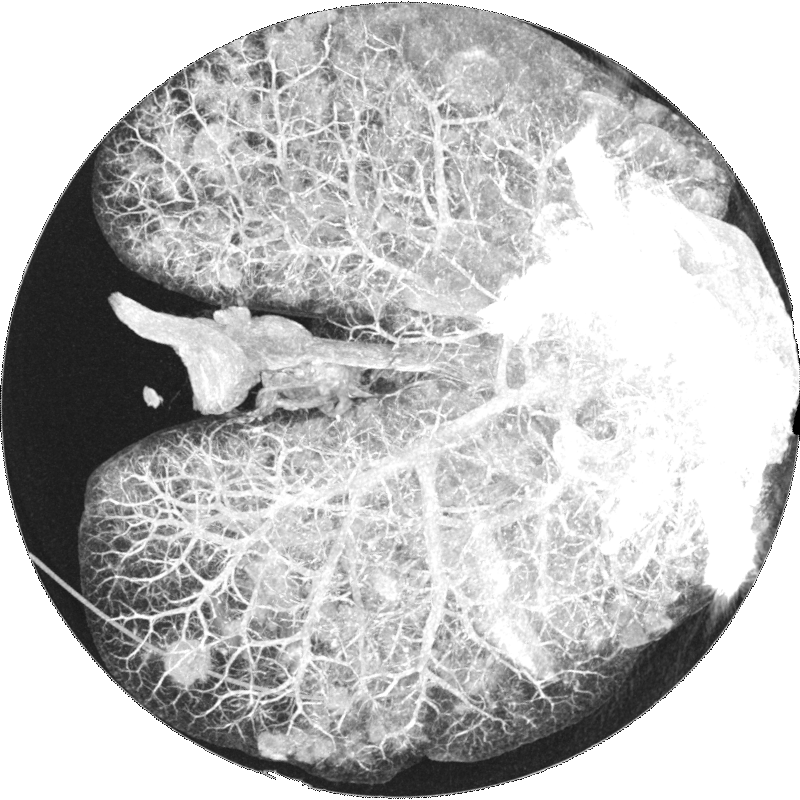
\includegraphics[width=\imsize]{../../Documents/Collaborations/DKF_Lung/Overview/MAX_wt13.png}%
\end{frame}

\begin{frame}{Tumor metastasis, Overview scan with \SI{20}{\micro\meter} pixel size}
    \centering
    \animategraphics[palindrome, width=0.5\linewidth]{12}{./img/tumor/mouse_tumor_rec0}{001}{263}
\end{frame}

\begin{frame}{Brain tumor radiation treatment}
    \begin{itemize}
        \item Induced tumors in rat brains
        \item Microbeam and broadbeam treatment vs.\ control
        \item \uaf-filled brain vasculature
        \item Nondestructive extraction of
        \begin{itemize}
            \item Vessel to tumor volume ratio
            \item Vessel surface
            \item Intra-tumoral microvessel density (IMD, \cite{Hasan2002})
        \end{itemize}
    \end{itemize}
\end{frame}

\begin{frame}{vessel volume ratio}
    \centering
    \includegraphics[width=\imsize]{../../Documents/Brain-Grenoble/fig/vessel_ratio_violin}
\end{frame}


\begin{frame}{vessel surface}
    \centering
    \includegraphics[width=\imsize]{../../Documents/Brain-Grenoble/fig/vessel_surface_per_tumor_volume}
\end{frame}

\begin{frame}{imd}
    \centering
    \includegraphics[width=\imsize]{../../Documents/Brain-Grenoble/fig/imd}
\end{frame}


\begin{frame}{References}
    \renewcommand*{\bibfont}{\tiny}
    \printbibliography
\end{frame}

\end{document}















\begin{frame}{Danio rerio}
\centering
\includegraphics[width=\imsize]{img/{{zebrafish_rec_voi_top_right}}}
%\begin{figure}%
%    \centering%
%    \pgfmathsetlength{\imagewidth}{\imsize}%
%    \pgfmathsetlength{\imagescale}{\imagewidth/1651}%
%    \def\x{1020}% scalebar-x starting at golden ratio of image width of 1651px = 1020
%    \def\y{391}% scalebar-y at 90% of image height of 434px = 391
%    \begin{tikzpicture}[x=\imagescale,y=-\imagescale]%
%        \node[anchor=north west, inner sep=0pt, outer sep=0pt] at (0,0) {\includegraphics[width=\imagewidth]{img/{{zebrafish_rec_voi_top_right}}}};
%        % 1615px = 35.48 > 100px = 2198um > 23px = 500um, 5px = 100um
%        %\draw[|-|,blue,thick] (20,154) -- (1634,127) node [sloped,midway,above,fill=white,semitransparent,text opacity=1] {\SI{35.487480000000005}{\milli\meter} (1615px) TEMPORARY!};
%        \draw[|-|,ultra thick] (\x,\y) -- (\x+234.19,\y) node [midway,above] {\SI{5}{\milli\meter}};
%    \end{tikzpicture}%
%    \caption{Visualization of a tomographic scan of a zebrafish, fixed in \SI{4}{\percent} PFA.}%
%\end{figure}%
\end{frame}

\begin{frame}
	\centering
	Examples
	 
\end{frame}

\end{document} 
